\documentclass{article}
\usepackage[utf8]{inputenc}
\usepackage{graphicx}
\usepackage{enumitem}
\usepackage{siunitx}
\usepackage{multirow}
\usepackage[a4paper, total={6in, 8in}]{geometry}
\usepackage[style=authoryear-ibid,backend=biber]{biblatex}
\usepackage[swedish]{babel}
\usepackage{float}
\usepackage{caption}
\usepackage[parfill]{parskip}
\usepackage{amsmath}
\usepackage{csquotes}
\usepackage{comment}
\usepackage{url}


\graphicspath{ {img/} }

\title{\Huge Operating Systems - Study \\ EDAF35}
%\author{\Large Elias Bergström, Emma Lindh, Elin Helmersson, Shahriar Chegini}
\author{  
    Elias Bergström\\
    \texttt{el8025be-s@student.lu.se}
    }
%\date{VT2024}
\date{\today}

\renewcommand{\figurename}{Figur}
\renewcommand{\tablename}{Tabell}

%handledarens namn

\begin{document}

\maketitle
\thispagestyle{empty}
%\pagenumbering{gobble}
\pagebreak
%\thispagestyle{empty}
%\pagenumbering{arabic}

\section{Module 2 - Processes and Threads}
\subsection{Red Box}
\begin{itemize}
    \item It is important to understand what the PCB is and that the PCBs get put on different queues by the OS when
    managing process state.
    (From section 3.1.3 to the end of 3.2.1 in Operating System Concepts)
    \item You need to understand process creation (including fork() and exec() in detail) and process termination (including
    zombie and orphan processes). From section 3.1.3 to the end of 3.2.1 in Operating System Concepts)
    \item You need to understand the difference between user threads and kernel threads and the different models for
    mapping between the two (Section 4.3 in Operating System Concepts)
\end{itemize}

\subsection{Notes}



The process can be in a number of different states, see figure.

\begin{figure}[H]
    \centering
    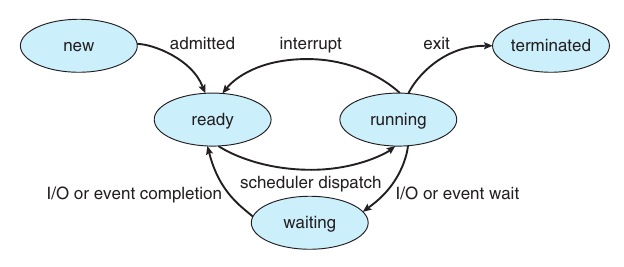
\includegraphics[width=0.8\textwidth]{pcb.png}
    \caption{Diagram of process states}
    \label{fig:diapcb}
\end{figure}


\subsubsection{PCB}
PCB stands for Process Control Block and each process is represented in the OS by one. The PCB contains information about the process:
\begin{itemize}
    \item {\bf Process state.} The state may be new, ready, running, waiting, halted, and
    so on.
    \item {\bf Program counter.} The counter indicates the address of the next instruction
    to be executed for this process.
    \item {\bf CPU registers.}
    \item {\bf CPU-scheduling information.} This information includes a process prior-
    ity, pointers to scheduling queues, and any other scheduling parameters.
    (Chapter 5 describes process scheduling.)
    \item {\bf Memory-management information.} This information may include such
    items as the value of the base and limit registers and the page tables, or the
    segment tables, depending on the memory system used by the operating
    system (Chapter 9).
    \item {\bf Accounting information} This information includes the amount of CPU
    and real time used, time limits, account numbers, job or process numbers,
    and so on.
    \item {\bf I/O status information.} This information includes the list of I/O devices
    allocated to the process, a list of open files, and so on.
\end{itemize}
In brief, the PCB simply serves as the repository for all the data needed to start,
or restart, a process, along with some accounting data.

\subsection*{fork() and exec() in Unix/Linux Context}

In a Unix/Linux context, \texttt{fork()} and \texttt{exec()} are system calls used for process creation and management.

\subsubsection*{fork()}
The \texttt{fork()} system call creates a new process by duplicating the calling (parent) process. The new process is called the \textit{child} process. Both the parent and the child process continue executing from the point of the \texttt{fork()} call. The child process gets a copy of the parent’s memory space, but they have different Process IDs (PIDs). \texttt{fork()} returns:
\begin{itemize}
    \item \texttt{0} in the child process.
    \item The child’s PID in the parent process.
\end{itemize}

\subsubsection*{exec()}
The \texttt{exec()} family of functions (e.g., \texttt{execvp()}, \texttt{execp()}, etc.) replaces the current process’s memory space with a new program. After calling \texttt{exec()}, the process image is completely replaced, and the new program starts executing. This is commonly used after \texttt{fork()} when the child process needs to run a different program than the parent.

\subsubsection*{Typical Usage}
In typical usage:
\begin{enumerate}
    \item \texttt{fork()} is used to create a new process.
    \item \texttt{exec()} is used by the child (or parent) to replace its process image with a different program.
\end{enumerate}

Together, these calls enable the creation of new processes and the execution of different programs, which is fundamental for tasks like launching new applications or running shell commands.



\subsubsection{Multithreading Models}
These models describes how to map user thread to kernel threads. User threads are supported above the kernel and are managed without kernel support and the kernel threads are managed by the kernel.

\begin{itemize}
    \item {\bf Many-to-One Model}, all user threads are mapped to one kernel 
    thread, where the switching between threads are done by a thread library in user space (not by the kernel)
    It's efficient but if the current user threads hangs it will also hang the kernel thread.
    \item {\bf One-to-One Model}, maps each user thread to a kernel thread. Multiple threads can run at the same time. The problem with this model is that you need to create a kernel thread for each user thread.
    \item {\bf Many-to-Many}, multiplexs many user threads to a smaller or equal amount of kernel threads.
    \item {\bf Two-Level Model} mixing two of the models. 
\end{itemize}




\section{Module 3.A - CPU Scheduling}
\subsection{Red Box}
\begin{itemize}
    \item Make sure you understand what it means for scheduling to be pre-emptive.
    (From section 5.1.3 in Operating System Concepts)
    \item You need to know and understand the tradeoffs between these different algorithms
    (Section 5.3 in Operating System Concepts)
    \item Be able to understand the differences between process and system contention scopes
    (Section 5.4 in Operating System Concepts)
    \item You need to understand ready queues, load balancing and processor affinity in multiprocessor systems
    (Section 5.5.1, 5.5.3 and 5.5.4 ins Operating System Concepts)
    \item You need to understand what makes real time scheduling different, the periodic process model and the
    differences between the RMS and the EDF scheduler (Section 5.6.1 – 5.6.4 in Operating System Concepts)
\end{itemize}

\begin{enumerate}
    \item When a process switches from the running state to the waiting state (for
    example, as the result of an I/O request or an invocation of wait() for the
    termination of a child process)
    \item When a process switches from the running state to the ready state (for
    example, when an interrupt occurs)
    \item When a process switches from the waiting state to the ready state (for
    example, at completion of I/O)
    \item When a process terminates
\end{enumerate}

When scheduling takes place only under circumstances 1 and 4, we say that the scheduling scheme is non preemptive or cooperative.
Otherwise, it is {\bf preemptive}. 
\\
\\
Chatgpt says the following:
\\ {\it Preemptive scheduling is a CPU scheduling method where the operating system can interrupt a running process to give the CPU to another process, usually with higher priority or urgency.
In this system, the OS can stop a process and switch to another one, either after a fixed time slice (in round-robin scheduling) or if a higher-priority process needs the CPU.}

\subsection{Scheduling Algorithms}

\subsubsection{First-Come, First-Served Scheduling (FCFS)}
This is the simplest algorithm. With this scheme, the process that requests the
CPU first is allocated the CPU first. The implementation of the FCFS policy is
easily managed with a FIFO queue. When a process enters the ready queue, its
PCB is linked onto the tail of the queue. When the CPU is free, it is allocated to
the process at the head of the queue. The running process is then removed from
the queue. The code for FCFS scheduling is simple to write and understand.
On the negative side, the average waiting time under the FCFS policy is
often quite long. {\bf Pro: simplest Con: Can have long wait times}.

\subsubsection{Shortest-Job-First (SJF) Scheduling}
Do the shortest job first. If to jobs take the same time FCFS is used to break the tie.
The more appropriate term for this method is {\bf shortest-next-CPU-burst}, because scheduling depends on the length of the next CPU burst of
a process, rather than its total length. 


% Problem here!
Although the SJF lagorithm is optimal, it cannot be implemented at the level of CPU scheduling, 
as there is no way to know the length of the next CPU burst.
One approach to this problem is to try to approximate SJF scheduling. We may
not know the length of the next CPU burst, but we may be able to predict its
value. We expect that the next CPU burst will be similar in length to the previous
ones. By computing an approximation of the length of the next CPU burst, we
can pick the process with the shortest predicted CPU burst.



{\bf Pro: less down time then FCFS Con: harder to implement.}

 
{\bf Whats the difference between Job and CPU burst?}

%Problem ends here!

\subsubsection{Round-Robin (RR) Scheduling}

Similar to FCFS but with preemption added. 

To implement RR scheduling, we again treat the ready queue as a FIFO
queue of processes. New processes are added to the tail of the ready queue.
\\
The CPU scheduler picks the first process from the ready queue, sets a timer to
interrupt after 1 time quantum, and dispatches the process.
One of two things will then happen. The process may have a CPU burst of
less than 1 time quantum. In this case, the process itself will release the CPU
voluntarily. The scheduler will then proceed to the next process in the ready
queue. If the CPU burst of the currently running process is longer than 1 time
quantum, the timer will go off and will cause an interrupt to the operating
system. A context switch will be executed, and the process will be put at the
tail of the ready queue. The CPU scheduler will then select the next process in
the ready queue.
\\

{\bf Con: the average waiting time under RR is often long. Pro: Relatively simple.}


\subsubsection{Priority Scheduling}

SJF is a special case of the general priority-scheduling. 
\\
A priority is associated with each process, and the CPU is allocated to the process with the highest priority. Equal-priority processes are scheduled in
FCFS order. An SJF algorithm is simply a priority algorithm where the priority
(p) is the inverse of the (predicted) next CPU burst. The larger the CPU burst,
the lower the priority, and vice versa.
\\


{\bf Con: different systems have different levels of priority, i.e. code is not portable.}



\subsubsection{Multilevel Queue Scheduling}

Separate queues for different priority levels. Often use RR per queue.
\\
{\bf Pro: you don't need to do an O(n) search to find the task with the highest priority.}



\subsubsection{Multilevel Feedback Queue Scheduling}

It's the same as Multilevel Queue Scheduling, but tasks can move between queues. 


%the differences between process and system contention scopes
\subsection{Contention Scope} %page 217


\subsection{}




\section{Module 3.B - Synchronization}
\subsection{Red Box}
\begin{itemize}
    \item You should know what the critical section problem is (Section 6.2 in Operating System Concepts)
    \item You must know the differences between Spinlocks, Semaphores and Mutexes in the context of Operating
    (Systems. 6.5 and 6.6 in Operating System Concepts – not the clearest explanation. Chapter 9, 10 in Linux Kernel
    development )
\end{itemize}


\subsection{Module 4 - Memory Management}
\subsubsection{Red Box}
\begin{itemize}
    \item YOU NEED TO UNDERSTAND WHAT THE PHYSICAL AND LOGIC ADDRESS SPACE IS AND THE MOTIVATION BEHIND IT. YOU ALSO NEED TO UNDERSTAND THAT
    THE MMU IS REQUIRED TO TRANSLATE BETWEEN THE TWO (9.1.1 TO 9.1.4 IN OPERATING SYSTEM CONCEPTS
    \item YOU NEED TO UNDERSTAND WHAT CONTIGOUS ALLOCATION IS, HOW IT WORKS AND WHY FRAGMENTATION IS A MAJOR ISSUE.
    (SECTION 9.2 IN OPERATING SYSTEM CONCEPTS)
    \item YOU NEED TO UNDERSTAND WHAT PAGING IS, WHAT THE PAGE TABLE AND TLB ARE, AND HAVE A GENERAL IDEA OF WHAT PROTECTION AND SHARED
    PAGES ARE (SECTION 9.2 IN OPERATING SYSTEM CONCEPTS
    \item YOU NEED TO KNOW WHY WE CANNOT USE SIMPLE PAGE TABLES, THE THREE ALTERNATIVE PAGE TABLE STRUCTURES AND THE ADVANTAGES AND
    DISADVANTAGES OF EACH (SECTION 9.4 OF OPERATING SYSTEM CONCEPTS
    \item YOU NEED TO UNDERSTAND THE BASIC CONCEPTS OF VIRTUAL MEMORY AND ITS ADVANTAGES(SECTION 10.1 OF OPERATING SYSTEM CONCEPTS)
    \item YOU NEED TO BE ABLE TO EXPLAIN WHAT DEMAND PAGING IS, FREE FRAME LIST AND ITS PERFORMANCE (SECTION 10.2 OF OPERATING SYSTEM CONCEPTS
    \item YOU NEED TO KNOW WHAT PAGE REPLACEMENT IS, UNDERSTAND THE MAIN THREE DIFFERENT PAGE REPLACEMENT ALGORITHMS DISCUSSED IN THE BOOK
    AND THEIR TRADEOFFS, AND BE ABLE TO DESCRIBE BELADY’S ANOMALY (SECTION 10.4 OF OPERATING SYSTEM CONCEPTS
\end{itemize}



\subsection{Module 4 pt 2 - Memory Management Additional Slides}
\subsubsection{Red Box}
\begin{itemize}
    \item YOU NEED TO KNOW THE CHALLENGES WITH ALLOCATING MEMORY IN THE OPERATING SYSTEM AND THE DIFFERENCES BETWEEN THE SLAB AND THE BUDDY
    ALLOCATER (SECTION 10.8 OF OPERATING SYSTEM CONCEPTS)
\end{itemize}


\subsection{Module 6 - File System}
\subsubsection{Red Box}
\begin{itemize}
    \item You should understand these two different access methods (13.2.1 and 13.2.2 in Operating System Concepts)
    \item You should understand what directories are and how they make it possible to organise and access files (13.3 in
    Operating System Concepts)
    \item This structure is discussed in the textbook but not very clearly. Try and understand it, but we will not ask
    questions discussing it directly (Section 14.1 in Operating System Concepts).
    \item Need to that know that files are represented as blocks and what the FCB/Inode is (Section 14.1 in Operating
    System Concepts).
    \item Need to understand what these two tables are and how calls like open() and read() use and update this table
    (Section 14.2.2 in Operating System Concepts)
    \item Understand these three different allocation methods and their relative advantages and disadvantages (Section
    14.4 in Operating System Concepts)
    \item Be able to calculate maximum file size a scheme like this can store (Section 14.4.3 in Operating System Concepts)
    \item Understand these two algorithms and their advantages and disadvantages (Section 14.5.1 and 14.5.2 in
    Operating System Concepts)
\end{itemize}


\subsection{Module 6 - I/O Systems}
\subsubsection{Red Box}
\begin{itemize}
    \item Need to be able to know what memory mapped I/O is and the motivation for why we use. (Section 12.2.1 in
    Operating System Concepts)
    \item You need to understand how these three different methods work and the motivations for each. (Section 12.2.2,
    12.2.3 and 12.2.4 in Operating System Concepts)
    \item You need to understand the differences and needs for these different interfaces. (Section 12.3.1 to 12.3.4 in
    Operating System Concepts)
    \item Make sure you understand this flow as it encompasses most of what we have spoken about today. (Section 12.5
    in Operating System Concepts)
\end{itemize}


\subsection{Module 7 - Protection and Security}
\subsubsection{Red Box!}
\begin{itemize}
    \item You should be able to describe what a domain of protection is and give examples of some different domains and
    objects (Section 17.4 in Operating System Concepts)
    \item You should be able to describe what the access matrix is, how it relates to domains of protection and how it can be implemented – you will not be asked about
    the lock and key mechanism, and only on the basics of capability lists (Section 17.5 and 17.6 in Operating System Concepts)
    \item Maintaining system security is very complicated and understanding this could require a whole courses – you will
    not be asked on this in the exam
\end{itemize}



\subsection{Module 8 - Virtualisation and Virtual Machines}
\subsubsection{Red Box}
\begin{itemize}
    \item You should know what virtualisation means and be able to briefly describe a few types of virtualisation eg: VMs,
    Virtual Networks, Virtual Disks and Virtual Memory
    \item You need to know the difference between different types of VMs: Type 1 and 2 hypervisors (not type 0
    hypervisors), Emulation and Containers. (Section 18.5.3, 18.5.4, 18.5.7 and 18.5.8 in Operating System Concepts)
\end{itemize}


\end{document}
